\documentclass{beamer}
\setbeamertemplate{footline}[page number]
\date{}
\author{}
\institute{}

%%%%%%% Put these names back in the final version 
%\\Aswathy Rajendra Kurup\\Meenu Ajith}
%\institute{Department of Electrical and Computer Engineering\\The University of New Mexico}
\setbeamercovered{transparent}
\usepackage{setspace}
\usepackage{array}
\usepackage[T1]{fontenc}
\usepackage{graphicx}
\usepackage{amsmath}
\usepackage{amsfonts}
\usepackage{amssymb}
\usepackage{makeidx}
\usefonttheme{serif}
\usepackage{multirow}
\usepackage{booktabs} 
\usepackage{rotating}
\usepackage{color}
\usepackage{float}
\usepackage[latin1]{inputenc}
\usepackage[english]{babel}
\usepackage{amsmath}
\usepackage{amsfonts}
\usepackage{eurosym}
\usepackage{rotating}
\usepackage{multicol}
\usepackage{pythonhighlight}
\usepackage[normalem]{ulem}
\newcommand{\ba}{{\bf a}}
\newcommand{\bb}{{\bf b}}
\newcommand{\bc}{{\bf c}}
\newcommand{\bd}{{\bf d}}
\newcommand{\be}{{\bf e}}
\newcommand{\bbf}{{\bf f}}
\newcommand{\bg}{{\bf g}}
\newcommand{\bh}{{\bf h}}
\newcommand{\bi}{{\bf i}}
\newcommand{\bk}{{\bf k}}
\newcommand{\bl}{{\bf l}}
\newcommand{\bm}{{\bf m}}
\newcommand{\bn}{{\bf n}}
\newcommand{\bo}{{\bf o}}
\newcommand{\bp}{{\bf p}}
\newcommand{\bq}{{\bf q}}
\newcommand{\br}{{\bf r}}
\newcommand{\bs}{{\bf s}}
\newcommand{\bt}{{\bf t}}
\newcommand{\bu}{{\bf u}}
\newcommand{\bv}{{\bf v}}
\newcommand{\bw}{{\bf w}}
\newcommand{\bx}{{\bf x}}
\newcommand{\by}{{\bf y}}
\newcommand{\bz}{{\bf z}}

\newcommand{\bA}{{\bf A}}
\newcommand{\bB}{{\bf B}}
\newcommand{\bC}{{\bf C}}
\newcommand{\bE}{{\bf E}}
\newcommand{\bG}{{\bf G}}
\newcommand{\bH}{{\bf H}}
\newcommand{\bI}{{\bf I}}
\newcommand{\bK}{{\bf K}}
\newcommand{\bL}{{\bf L}}
\newcommand{\bM}{{\bf M}}
\newcommand{\bO}{{\bf O}}
\newcommand{\bQ}{{\bf Q}}
\newcommand{\bR}{{\bf R}}
\newcommand{\bS}{{\bf S}}
\newcommand{\bT}{{\bf T}}
\newcommand{\bV}{{\bf V}}
\newcommand{\bW}{{\bf W}}
\newcommand{\bX}{{\bf X}}
\newcommand{\bY}{{\bf Y}}
\newcommand{\bZ}{{\bf Z}}
\newcommand\uptocnt{\stackrel{\mathclap{\normalfont\mbox{c}}}{\propto}}
\newcommand{\bpt}{{\bf pt}}
\newcommand{\bpl}{{\bf pl}}
\newcommand{\bdp}{{\bf dp}}
\newcommand{\btemp}{{\bf temp}}

\newcommand{\bmu}{{\boldsymbol \mu}}
\newcommand{\bSigma}{{\boldsymbol \Sigma}}
\newcommand{\bsigma}{{\boldsymbol \sigma}}
\newcommand{\bvarPhi}{{\boldsymbol \varPhi}}
\newcommand{\bvarphi}{{\boldsymbol \varphi}}
\newcommand{\bPhi}{{\boldsymbol \Phi}}
\newcommand{\bdelta}{{\boldsymbol \delta}}
\newcommand{\bZero}{{\bf 0}}
\newcommand{\bOne}{{\bf 1}}
\newcommand{\balpha}{{\boldsymbol \alpha}}
\newcommand{\bAlpha}{{\boldsymbol A}}
\newcommand{\btheta}{{\boldsymbol \theta}}

\newcommand{\softmax}{\text{softmax}}
\newcommand{\diag}{\text{diag}}
\newcommand{\sinc}{\mathrm{sinc}}
\newcommand{\argmin}{\mathop{\mathrm{argmin}}}
\newcommand{\infl}{\eta}
\newcommand{\Ind}{\mathrm{I}}
\newcommand{\Real}{\mathbb R}
\newcommand{\Intg}{\mathbb Z}
\newcommand{\Complex}{\mathbb C}
\newcommand{\Natural}{\mathbb N}
\newcommand{\Fourier}[1]{\mathcal{F} \{#1\}}
%\newcommand{\ii}{\mathbbm{i}}
\newcommand{\bphi}{\boldsymbol{\mathit{\phi}}}

\newcommand{\hs}{\hspace{2pt}}
\newcommand{\sign}{\text{sign}}
\author{Manel Mart\'inez-Ram\'on\\Meenu Ajith\\Aswathy Rajendra Kurup}

\usetheme{Madrid}
\usecolortheme{beaver}
\usepackage{tikz}
\usetikzlibrary{fit,arrows,calc,positioning}
\usepackage{listings}
\usepackage{xcolor}
\usepackage{emerald} 
\usepackage[T1]{fontenc} 
\usepackage{verbatim}
\usepackage{graphicx}
\usepackage{epsfig}
\usepackage{psfrag}
\usepackage[english]{babel}
\usepackage{listings}
\usepackage{courier}
\usepackage{color}
 \usepackage{vwcol} 
 \usepackage[english]{babel} % To obtain English text with the blindtext package
\usepackage{blindtext}
\definecolor{codegreen}{rgb}{0,0.6,0}
\definecolor{codegray}{rgb}{0.5,0.5,0.5}
\definecolor{codepurple}{rgb}{0.58,0,0.82}
\definecolor{backcolour}{rgb}{0.95,0.95,0.92}

\lstdefinestyle{mystyle}{
  backgroundcolor=\color{backcolour},   commentstyle=\color{codegreen},
  keywordstyle=\color{magenta},
  numberstyle=\tiny\color{codegray},
  stringstyle=\color{codepurple},
  basicstyle=\ttfamily\footnotesize,
  breakatwhitespace=false,         
  breaklines=true,                 
  captionpos=b,                    
  keepspaces=true,                 
  numbers=left,                    
  numbersep=5pt,                  
  showspaces=false,                
  showstringspaces=false,
  showtabs=false,                  
  tabsize=2
}
\lstset{style=mystyle}

%% Stuff for movies

% %\newcommand{\bt}{{\bf t}}
% \newcommand{\br}{{\bf r}}
% \newcommand{\bs}{{\bf s}}
% \newcommand{\by}{{\bf y}}
% \newcommand{\bz}{{\bf z}}
% \newcommand{\bx}{{\bf x}}
% \newcommand{\bw}{{\bf w}}
% \newcommand{\be}{{\bf e}}
% \newcommand{\bbf}{{\bf f}}
% \newcommand{\bb}{{\bf b}}
% \newcommand{\bd}{{\bf d}}
% \newcommand{\bA}{{\bf A}}
% \newcommand{\bB}{{\bf B}}
% \newcommand{\bL}{{\bf L}}
% \newcommand{\bM}{{\bf M}}

% \newcommand{\bC}{{\bf C}}
% \newcommand{\bI}{{\bf I}}
% \newcommand{\bK}{{\bf K}}
% \newcommand{\bk}{{\bf k}}
% \newcommand{\bT}{{\bf T}}
% \newcommand{\bV}{{\bf V}}
% \newcommand{\bW}{{\bf W}}
% \newcommand{\bX}{{\bf X}}
% \newcommand{\bY}{{\bf Y}}
% \newcommand{\bZ}{{\bf Z}}
% \newcommand{\bm}{{\bf m}}
% \newcommand{\bpt}{{\bf pt}}
% \newcommand{\bpl}{{\bf pl}}
% \newcommand{\bdp}{{\bf dp}}
% \newcommand{\btemp}{{\bf temp}}
% \newcommand{\bl}{{\bf l}}
% \newcommand{\bu}{{\bf u}}
% \newcommand{\bmu}{{\boldsymbol \mu}}
% \newcommand{\bSigma}{{\boldsymbol \Sigma}}
% \newcommand{\bLambda}{{\boldsymbol \Lambda}}

% \newcommand{\bsigma}{{\boldsymbol \sigma}}
% \newcommand{\bvarphi}{{\boldsymbol \varPhi}}
% \newcommand{\btheta}{{\boldsymbol \theta}}
% \newcommand{\bZero}{{\bf 0}}
% \newcommand{\balpha}{{\boldsymbol \alpha}}
% \newcommand{\bpi}{{\boldsymbol \pi}}
% \newcommand{\bxi}{{\boldsymbol \xi}}
% \newcommand{\bdelta}{{\boldsymbol \delta}}
\lstset{
	language=Python,
	basicstyle=\footnotesize\ttfamily\color{black},
	commentstyle = \footnotesize\ttfamily\color{red},
	keywordstyle=\footnotesize\ttfamily\color{blue},
	stringstyle=\footnotesize\ttfamily\color{black},
%	columns=fixed,
%	numbers=left,    
	numberstyle=\tiny,
	stepnumber=1,
	numbersep=5pt,
	tabsize=1,
	extendedchars=true,
	breaklines=true,            
	frame=b,         
	showspaces=false,
	showtabs=true,
	xleftmargin=6pt,
	framexleftmargin=6pt,
	framexrightmargin=2pt,
	framexbottommargin=4pt,
	showstringspaces=false      
}

\lstloadlanguages{
         Python
}

%\graphicspath{ {./images/} }  % Figures path - used in graphicx

%\selectcolormodel{cmyk}

\mode<presentation>

\newcommand{\dred}{darkred!90!black}
\newcommand{\written}{\ECFJD\textcolor{cyan!50!white}}
\newcommand{\hlight}{\textcolor{\dred}}
\newcommand{\Ex}{\textcolor{\dred}{Ex. }}

% remove navigation symbols in full screen mode
\setbeamertemplate{navigation symbols}{}  
\setbeamertemplate{blocks}[rounded][shadow=false]
\setbeamercolor{note page}{fg=black}

\setbeamercolor{title}{fg=\dred}
\setbeamercolor{frametitle}{fg=white}
\setbeamercolor{frametitle}{bg=\dred}
\setbeamercolor{structure}{fg=black,bg=white}
\setbeamercolor{background canvas}{bg=white,fg=black}
\setbeamercolor{normal text}{fg=black,bg=white}
\setbeamercolor{item}{fg=red!80!black,bg=white!}
\addtobeamertemplate{block begin}{\setbeamercolor{block title}{fg=white,bg=\dred}
\setbeamercolor{block body}{fg=white,bg=gray}}{}



\title{3. Deep Learning tools}
\subtitle{3.5 Scikit-learn}

\addtobeamertemplate{frametitle}{}

\begin{document}

\maketitle
\begin{frame}{Introduction}
   \begin{itemize}  
   \item Scikit-learn is a free machine learning library in Python developed  by David Cournapeau as a Google Summer of Code project in 2007.
   \item It has various features for pre-processing, model selection, classification, clustering, regression and dimensionality reduction. 
   \item It is built on top of NumPy, SciPy and Matplotlib. 
   \end{itemize}
\end{frame}


\begin{frame}[fragile]{The Scikit-Learn API}

\begin{itemize}
\item The API has three interfaces that do most of the ML tasks. It also has pre-built algorithms. 
 
\begin{itemize}
 \item[]\textbf{Estimator:}  It uses the \emph{fit()} method to train the machine learning model. All regression, classification or unsupervised tasks use the estimator interface.
 
 \item[]\textbf{Predictor} It uses
the \emph{predict()} method to make  predictions on test features. A single \emph{fit\_predict()} method can be used.
 
 \item[]\textbf{Transformer} The \emph{transform()} method provides a library of transformations for data preprocessing, dimensionality reduction, feature extraction, and feature selection. The \emph{fit\_transform()} models and transforms the training data simultaneously.
\end{itemize}
\end{itemize}
\end{frame}



\begin{frame}[fragile]{Datasets}
\begin{itemize}
    \item Toy examples, real data and data generators can be used with the library.
    \item Here are some examples:
\end{itemize}

\begin{lstlisting}
#LOADING THE TOY DATSET
from sklearn import datasets
data = datasets.load_wine() #Load the wine dataset.
#LOADING REAL-WORLD DATASET
from sklearn.datasets import fetch_california_housing
house_data = fetch_california_housing() # A housing dataset.

#LOADING GENERATED DATASET
from sklearn.datasets import make_blobs
#Develop isotropic Gaussian blobs for clustering.
X, y = make_blobs(n_samples=60, centers=3, n_features=3, random_state=0) 

\end{lstlisting}

\begin{verbatim}
\end{verbatim}
\end{frame}



\begin{frame}[fragile]{Making blobs}
\begin{lstlisting}
from sklearn.datasets import make_blobs
X, y = make_blobs(n_samples=200, centers=3, n_features=2, random_state=0) 
\end{lstlisting}

\begin{multicols}{2}

\begin{lstlisting}
string=['*r','+k','ob']
for j in range(3):
  ind = np.where(y==j)
  plt.plot(X[ind,0],X[ind,1],string[j])
plt.show()
\end{lstlisting}

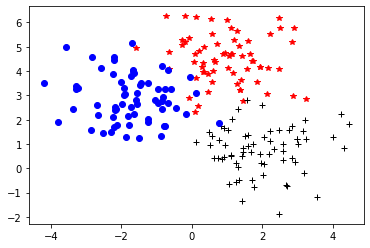
\includegraphics[scale=0.45]{Module 2 (Python tools)/pics/blobs.png}

\end{multicols}

\end{frame}

\begin{frame}{Preprocessing}



\begin{table}[H]
\begin{tabular}{|l|l|}
\hline
\multicolumn{1}{|c|}{\textbf{Methods}} & \multicolumn{1}{c|}{\textbf{Functions}}                                                                                                                                                                                                             \\ \hline
Standardization                                      & \begin{tabular}[c]{@{}l@{}}StandardScaler()-Zero mean, unit var.\\ MinMaxScaler()- Between $a$ and $b$.\end{tabular}                                                      \\ \hline
Normalization                                        & \begin{tabular}[c]{@{}l@{}}Normalizer()-unit norm.\end{tabular}                                                                                                                                                \\ \hline
Imputing values                                      & \begin{tabular}[c]{@{}l@{}}SimpleImputer()-  Fills up missing values \\ Mean, most frequent, median,  constant.\end{tabular}                                                                           \\ \hline
Polynomial Features                                  & \begin{tabular}[c]{@{}l@{}}PolynomialFeatures()- Adds complexity\\ by generating polynomial features.\end{tabular}                                                                                                                  \\ \hline
Categorical Features                                 & \begin{tabular}[c]{@{}l@{}}OneHotEncoder()- Categorical encoding.\\  OrdinalEncoding()- Encodes unique cats.\\  \end{tabular} \\ \hline
Numerical Features                                   & \begin{tabular}[c]{@{}l@{}}KBinsDiscretizer()- Real to discrete bins.\\ Binarizer()- Thresholds numerical features.\end{tabular}                     \\ \hline
Custom Transformers                                  & \begin{tabular}[c]{@{}l@{}}FunctionTransformers()- Accepts an existing \\ function and uses it to transform the data.\end{tabular}                                                                                                                  \\ \hline
\end{tabular}
\caption{Data preprocessing methods and functions}
\label{table:1}
\end{table}
\end{frame}



\begin{frame}[fragile]{Preprocessing}
\begin{itemize}
    \item A preprocessing example that does data imputation
\end{itemize}

\begin{lstlisting}
#IMPUTING VALUES
import numpy as np
from sklearn.impute import SimpleImputer
arr3 = np.array([[np.nan, 2, 8, np.nan], [6, np.nan, np.nan, 12], [7, 6, 4, np.nan]]) #define an array.
print("Original array:",arr3)
im = SimpleImputer(missing_values=np.nan, strategy='median') #define the preprocessing module.
arr_im = im.fit_transform(arr3) #fills the missing data.
print("Array after imputing values:",arr_im)
\end{lstlisting}
\begin{small}
\begin{verbatim}
Original array: [[nan  2.  8. nan]
 [ 6. nan nan 12.]
 [ 7.  6.  4. nan]]
Array after imputing values: [[ 6.5  2.   8.  12. ]
 [ 6.   4.   6.  12. ]
 [ 7.   6.   4.  12. ]]
\end{verbatim}
\end{small}
\end{frame}

\begin{frame}[fragile]{Feature selection and machine learning}
\begin{itemize}
    \item \textbf{Feature selection:} Scikit-learn provides several feature selection algorithms. The most widely used methods are Recursive Feature Elimination (RFE) and SelectKBest. 
    \item \textbf{Learning models:} 
    \begin{itemize}
\item \textbf{Supervised:} The most commonly used supervised learning method includes linear models such as Linear regression, Logistic regression, Ridge regression, Lasso regression , Decision trees, Naive Bayes Classifier, Support Vector Machines, Random Forests, and others;  
\item \textbf{Unsupervised:} Isomap, t-SNE,  K-Means, Gaussian Mixture Models. 
\end{itemize}
\item Examples are provided in separate Jupyter notebooks.
\end{itemize}
\end{frame}

\end{document}	





\begin{frame}[fragile]{}
\begin{itemize}
    \item 
\end{itemize}

\begin{lstlisting}
\end{lstlisting}

\begin{verbatim}
\end{verbatim}
\end{frame}